\documentclass{article}
\usepackage{geometry}
\geometry{a4paper,scale=0.9}
\usepackage{pdfpages}
\usepackage{steinmetz}
\usepackage{ctex}
\usepackage{amsmath}
\usepackage[version=4]{mhchem}
\usepackage{graphicx}
\usepackage{xcolor}
\usepackage{longtable}
\usepackage{booktabs}
\usepackage[scr]{rsfso}
\newcommand{\Laplace}{\mathscr{L}}
\newcommand{\Fourier}{\mathscr{F}}
\usepackage{indentfirst}
\setlength{\parindent}{0pt}
\usepackage{listings}
\lstset{
	language=Matlab,
	frame=shadowbox, %把代码用带有阴影的框圈起来
  	rulesepcolor=\color{red!20!green!20!blue!20},%代码块边框为淡青色
  	keywordstyle=\color{blue!90}\bfseries, %代码关键字的颜色为蓝色,粗体
  	commentstyle=\color{red!10!green!70}\textit,    % 设置代码注释的颜色
 	 	showstringspaces=false,%不显示代码字符串中间的空格标记
  	numbers=left, % 显示行号
  	numberstyle=\tiny,    % 行号字体
  	stringstyle=\ttfamily, % 代码字符串的特殊格式
  	breaklines=true, %对过长的代码自动换行
  	extendedchars=false,  %解决代码跨页时,章节标题,页眉等汉字不显示的问题
  	escapebegin=\begin{CJK*}{GBK}{hei},escapeend=\end{CJK*},      % 代码中出现中文必须加上,否则报错
  	texcl=true
}
\renewcommand {\thetable} {\thesection{}.\arabic{table}}
\renewcommand {\thefigure} {\thesection{}.\arabic{figure}}

\title{Control System Note}
\author{Yizhen Wang}
\date{\today}

\begin{document}

\maketitle
\thispagestyle{empty}
\newpage
\thispagestyle{empty}
\section*{前言}

这篇笔记基于Katsuhiko Ogata所著的《现代控制工程》(第五版),内容与例图基本均来源于该书,仅作整理与总结归纳,供个人复习使用。
\tableofcontents
\thispagestyle{empty}
\newpage

\setcounter{page}{1}


\section{数学模型}

\subsection{拉普拉斯变换}

定义:

\begin{align*}
f(t)&=\mbox{时间$t$的函数,并且当$t<0$时$f(t)=0$}\\
s&=\mbox{复变量}\\
\Laplace&=\mbox{运算符号,表示该量用拉普拉斯积分$\int_0^\infty e^{-st}dt$进行变换}\\
F(s)&=f(t)\mbox{的拉普拉斯变换}
\end{align*}

于是,$f(t)$的拉普拉斯变换为

\begin{equation*}
\Laplace[f(t)]=F(s)=\int_0^\infty e^{-st}dt[f(t)]=\infty_0^\infty f(t)e^{-st}dt
\end{equation*}

从拉普拉斯变换$F(s)$求时间函数$f(t)$的反变换过程称为拉普拉斯反变换:

\begin{equation*}
\Laplace^{-1}[F(s)]=f(t)=\frac{1}{2\pi j}\int_{c-j\infty}^{c+j\infty}F(s)e^{st}ds
\end{equation*}

一般不通过计算反演积分来求拉普拉斯反变换,多数情况可以通过部分分式展开再查表来求$f(t)$。

初值定理:

\begin{equation*}
f(0+)=\lim_{t\to0+}f(t)=\lim_{s\to\infty}sF(s)
\end{equation*}

终值定理:

\begin{equation*}
f(\infty)=\lim_{t\to \infty}f(t)=\lim_{s\to0}sF(s)
\end{equation*}

在复平面上,使复变函数$G(s)$解析(满足柯西-黎曼条件)的点称为普通点,使其非解析的点称为奇点;使$G(s)$或其导数趋近于无穷大的奇点称为极点,使$G(s)$等于零的奇点称为零点。

$s$趋近于$p$时,$G(s)$趋于无穷大,且$G(s)(s-p)^n$在$s=p$处取到一个非零的有限值,则称该极点为$n$阶极点。

\subsection{傅里叶变换}

用$j\omega$代替拉普拉斯变换中的$s$,即可得到傅里叶变换,其中的$\omega$为频率,其单位为$rad/s$;当使用频率进行测量时,用$f$表示,$\omega=2\pi f$。

\begin{equation*}
F(j\omega)=\Fourier[f(t)]=\int_{-\infty}^\infty f(t)e^{-j\omega t}dt
\end{equation*}

对应的傅里叶逆变换:

\begin{equation*}
f(t)=\Fourier^{-1}[F(j\omega)]=\frac{1}{2\pi}\int_{-\infty}^\infty f(t)e^{j\omega t}d\omega
\end{equation*}



\subsection{传递函数}

对于微分方程

\begin{align*}
a_0y^{(n)}+a_1y^{(n-1)}&+\cdots+a_{n-1}\dot y+a_ny\\
&=b_0x^{(m)}+b_1x^{(m-1)}+\cdots+b_{m-1}\dot x+b_mx\hspace{2em}(n\ge m)
\end{align*}

式中,$x$为输入,$y$为输出,其对应的传递函数定义为输入与输出的拉普拉斯变换的比值:



\begin{equation*}
\begin{aligned}
\mbox{传递函数}&:=G(s)\\
&=\frac{\Laplace[\mbox{输出量}]}{\Laplace[\mbox{输入量}]}\Big|_{\mbox{零初始条件}}\\
&=\frac{Y(s)}{X(s)}\\
&=\frac{b_0s^m+b_1s^{m-1}+\cdots+b_{m-1}s+b_m}{a_0s^n+a_1s^{n-1}+\cdots+a_{n-1}+a_n}
\end{aligned}
\end{equation*}

传递函数中,如果分母$s$的最高阶次为$n$,则称系统为$n$阶系统。

\subsection{卷积积分}
由传递函数的定义,可以得到

\begin{equation*}
Y(s)=G(s)X(s)
\end{equation*}

由拉普拉斯变换的性质可知,复域内的乘法等价于时域内的卷积,因此有

\begin{align*}
y(t)&=\int_0^tx(\tau)g(t-\tau)d\tau\\
&=\int_0^tg(\tau)x(t-\tau)d\tau
\end{align*}

\subsection{脉冲响应函数}

同样地,由传递函数的定义可以知道,如果能找到一个输入函数,其拉普拉斯变换为$1$(准确来讲是单位阶跃函数$u(t)$),那么就能得到

\begin{equation*}
Y(s)=G(s)
\end{equation*}

此时需要的输入函数就应当是单位脉冲函数$\delta(t)$

\begin{equation*}
x(t)=\Laplace^{-1}[1]=\delta(t)
\end{equation*}

对输出量进行拉普拉斯反变换,得到的函数即称为脉冲响应函数,


\begin{equation*}
\Laplace^{-1}[G(s)]=g(t)
\end{equation*}

脉冲响应函数的意义是,当初始条件为$0$时,对系统输入一个单位脉冲函数,此时得到的输出。对这个脉冲响应函数作拉普拉斯变换,即可得到传递函数$G(s)$。

\subsection{闭环传递函数的等效}


\begin{figure}[!ht]
	\centering
	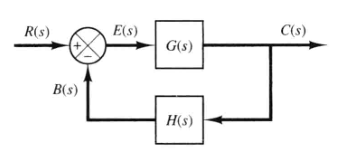
\includegraphics[width=8cm]{figures/2.png}
	\caption{闭环控制系统方块图}
	\label{2}
\end{figure}



如图\ref{2}所示的闭环控制系统,输出量$C(s)$与输入量$R(s)$之间的关系有
\begin{align*}
C(s)&=G(s)E(s)\\
E(s)&=R(s)-B(s)\\
&=R(s)-C(s)H(s)
\end{align*}

消去$E(s)$,从而有
\begin{align*}
C(s)&=G(s)[R(s)-H(s)C(s)]\\
[1+G(s)H(s)]C&=G(s)R(s)\\
\frac{C(s)}{R(s)}&=\frac{G(s)}{1+G(s)H(s)}
\end{align*}

这个式子可以消去反馈回路,化简方块图。

\subsection{非线性系统的线性化}

一个系统如果不能满足叠加原理,则该系统是非线性系统。但考虑到线性系统的优良性质,并且实际状况下,系统围绕着平衡点工作,将信号视为围绕平衡点变化的小信号,就可以用线性系统来近似非线性系统。对于非线性系统,输入为$u(t)$,输出为$y(t)$,满足关系

\begin{equation*}
	f(y^{(n)},y^{(n-1)},\cdots,y',y,u^{(m)},u^{(m-1)},\cdots,u',u)=0
\end{equation*}

线性化的具体的做法如下:

\begin{enumerate}
	\item 求平衡状态。令式中$u$和$y$的各阶导数均为0,结合给定的限制条件(对平衡位置的要求),得到平衡状态下的$\bar{u}$,$\bar{y}$:
	
	\begin{equation*}
		f(0,0,\cdots,0,\bar{y},0,0,\cdots,0,\bar{u})=0
	\end{equation*}

	\item 将原输入、输出$u$,$y$映射为新的变量$\delta_u$,$\delta_y$:
	
	\begin{align*}
		\delta_u&=u-\bar{u}\\
		\delta_y&=y-\bar{y}
	\end{align*}

	显然,对应的导数不发生变化:

	\begin{align*}
		\frac{d^k\delta_y}{dt^k}&=\frac{d^ky}{dt^k}\\
		\frac{d^k\delta_u}{dt^k}&=\frac{d^ku}{dt^k}
	\end{align*}

	\item 利用泰勒展开,只取第一项,得到对应的线性化系统(每项偏导均代入平衡状态下的取值)
	
	\begin{align*}
		&f(y^{(n)},y^{(n-1)},\cdots,y',y,u^{(m)},u^{(m-1)},\cdots,u',u)\\
		=&f(0,0,\cdots,0,\bar{y},0,0,\cdots,0,\bar{u})\\
		&\phantom{aaa}+\frac{\partial f}{\partial y^{(n)}}(y^{(n)}-0)+\frac{\partial f}{\partial y^{(n-1)}}(y^{(n-1)}-0)+\cdots+\frac{\partial f}{\partial y}(y-\bar{y})\\
		&\phantom{aaa}+\frac{\partial f}{\partial u^{(m)}}(u^{(m)}-0)+\frac{\partial f}{\partial u^{(m-1)}}(u^{(m-1)}-0)+\cdots+\frac{\partial f}{\partial u}(u-\bar{u})\\
		=&0+\frac{\partial f}{\partial y^{(n)}}\delta_y^{(n)}+\frac{\partial f}{\partial y^{(n-1)}}\delta_y^{(n-1)}+\cdots+\frac{\partial f}{\partial y}\delta_y\\
		&\phantom{aaa}+\frac{\partial f}{\partial u^{(m)}}\delta_u^{(m)}+\frac{\partial f}{\partial u^{(m-1)}}\delta_u^{(m-1)}+\cdots+\frac{\partial f}{\partial u}\delta_u\\
		=&f_{lin}(\delta_y^{(n)},\delta_y^{(n-1)},\cdots,\delta_y',\delta_y,\delta_u^{(m)},\delta_u^{(m-1)},\cdots,\delta_u',\delta_u)=0\\
	\end{align*}
\end{enumerate}




\subsection{用MATLAB求传递函数}

定义传递函数可以利用MATLAB中的\textit{tf}函数。例如,要定义传递函数

\begin{equation*}
	G(s)=\frac{s^2-2s+16}{3s+1}
\end{equation*}

可以这样来定义:

\begin{lstlisting}
s=tf('s');
sys{1}=(s^2-2*s+16)/(3*s+1)
\end{lstlisting}

此外,还可以通过函数\textit{step}和函数\textit{bode}来求取对应的阶跃响应和频响特性曲线。

\begin{figure}[!ht]
	\centering
	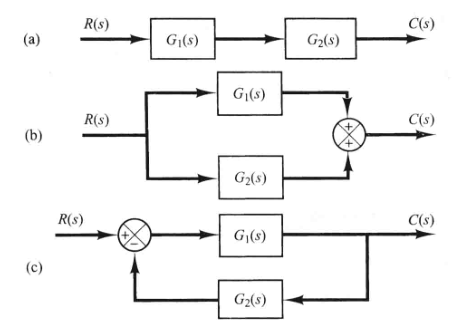
\includegraphics[width=8cm]{figures/1.png}
	\caption{串联、并联与闭环反馈}
	\label{1}
\end{figure}

对于串联、并联和闭环反馈形式的传递函数,如图\ref{1},可以用这样的MATLAB命令来定义:

\begin{lstlisting}
[num,den] = series(num1,den1,num2,den2)
[num,den] = parallel(num1,den1,num2,den2)
[num,den] = feedback(num1,den1,num2,den2)
\end{lstlisting}

比如,对于传递函数$G_1(s)$和$G_2(s)$的闭环反馈
\begin{equation*}
G_1(s)=\frac{10}{s^2+2s+10}=\frac{num1}{den1},\hspace{2em}G_2(s)=\frac{5}{s+5}=\frac{num2}{den2}
\end{equation*}

可以用下面的代码实现

\begin{lstlisting}
num1 = [10];
den1 = [1,2,10];
num2 = [5];
den2 = [1,5];
[num,den] = feedback(num1,den1,num2,den2);
printsys(num,den)
\end{lstlisting}
\section{机械系统的控制模型}
机械系统的基本定律是牛顿第二定律$F=ma$。
\subsection{弹簧}
\begin{figure}[!ht]
	\centering
	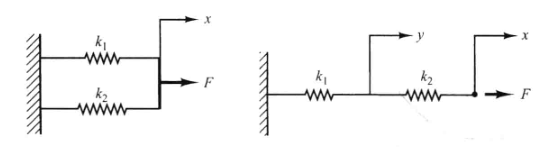
\includegraphics[width=8cm]{figures/3.png}
	\caption{并联与串联弹簧系统}
	\label{3}
\end{figure}

弹簧遵守胡克定律$F=kx$,如\ref{3}所示的并联与串联弹簧系统,其等效劲度系数为

\begin{align*}
k_{eq,parallel}&=k_1+k_2\\
\frac{1}{k_{eq,series}}&=\frac{1}{k_1}+\frac{1}{k_2}
\end{align*}

弹簧可以储贮存势能。

\subsection{阻尼器}

\begin{figure}[!ht]
	\centering
	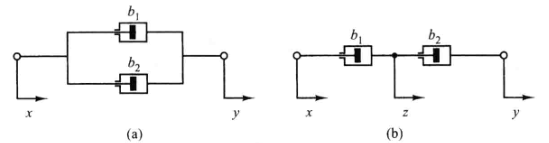
\includegraphics[width=8cm]{figures/4.png}
	\caption{并联与串联阻尼系统}
	\label{4}
\end{figure}

阻尼器可以阻碍相对运动,其提供摩擦力的大小与所连接的两物体间相对速度成正比,即$f=bv$,式中$b$称为粘性摩擦系数。如\ref{4}所示的串联与并联弹簧系统,其等效粘性摩擦系数为

\begin{align*}
b_{eq,parallel}&=b_1+b_2\\
\frac{1}{b_{eq,series}}&=\frac{1}{b_1}+\frac{1}{b_2}
\end{align*}

阻尼器不能贮存动能和势能。

\subsection{质量块}

质量块遵循牛顿第二定律,即$F=ma$。质量块可以贮存动能和势能。
\section{电路系统的控制模型}
电路系统(仅考虑集总参数电路)的基本定律是基尔霍夫定律(KCL与KVL)。
\subsection{电阻元件}
电阻元件遵循欧姆定律,且无法贮能。
\begin{equation*}
e=Ri
\end{equation*}

\subsection{电容元件}
电容元件的定义式为$C=q/{e}$,可以贮存电场能,由定义式可以得到
\begin{equation*}
e=\frac{1}{C}\int idt
\end{equation*}

\subsection{电感元件}
电感元件可以贮存磁场能,其两端电势差与电流间的关系遵循
\begin{equation*}
e=L\frac{di}{dt}
\end{equation*}

\subsection{串联元件的传递函数}

由于元件间的负载效应,元件间的串联会导致负载效应。即,单独分析电路的一部分时,所得到的传递函数相当于负载阻抗无穷大的情况,然而实际上,能量在输出端上存在损耗。因此,串联元件的传递函数,不能直接相乘得到。

对于无负载效应,或是负载效应可以忽略不计的电路,其传递函数可以通过单个电路传递函数的乘积得到。

\subsection{复阻抗}

复阻抗$Z(s)$的定义为,元件两端电压的拉普拉斯变换$E(s)$,与通过元件电流的拉普拉斯变换$I(s)$的比,

\begin{equation*}
Z(s):=\frac{E(s)}{I(s)}
\end{equation*}

从而,电阻的复阻抗仍然为$R$,电容的复阻抗变为$1/sC$,电感的复阻抗变为$sL$。利用复阻抗,可以把所有电路元件视为具有复阻抗的线性电阻元件,直接利用基尔霍夫定律推导出传递函数,无需再逐一列些微分方程、做拉普拉斯变换,为计算带来极大的方便。

\subsection{运算放大器}

理想运算放大器的性质:
\begin{itemize}
	\item	输入电压间的电势差为0,$v_+=v_-$
	\item	输入阻抗无穷大,因此输入电流为0,即$i_+=i_-=0$
\end{itemize}




\section{瞬态响应和稳态响应分析}
\subsection{瞬态响应和稳态响应}
\begin{itemize}
	\item	瞬态响应:系统从初始状态到最终状态的响应过程
	\item	稳态响应:系统在时间$t$趋于无穷大时的系统输出状态
\end{itemize}

系统响应可表示为
\begin{equation*}
c(t)=c_{tr}(t)+c_{ss}(t)
\end{equation*}

其中,$c_{tr}(t)$为瞬态响应(transient),$c_{ss}(t)$为稳态响应(steady-state)。

\subsection{一阶系统}

\begin{figure}[!ht]
	\centering
	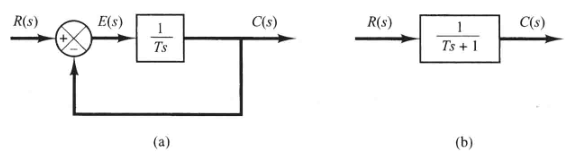
\includegraphics[width=8cm]{figures/5.png}
	\caption{一阶系统}
	\label{5}
\end{figure}

如图\ref{5},一阶系统的传递函数为

\begin{equation*}
G(s)=\frac{C(s)}{R(s)}=\frac{1}{1+Ts}
\end{equation*}

\subsubsection{单位阶跃响应}

单位阶跃响应的拉普拉斯变换为$1/s$,代入得到

\begin{equation*}
C(s)=\frac{1}{1+Ts}\frac{1}{s}=\frac{1}{s}-\frac{1}{s+\frac1T}
\end{equation*}

对上式作拉普拉斯反变换,有

\begin{equation*}
c(T)=\Laplace^{-1}C(s)=1-e^{-{t}/{T}}
\end{equation*}

\begin{figure}[!ht]
	\centering
	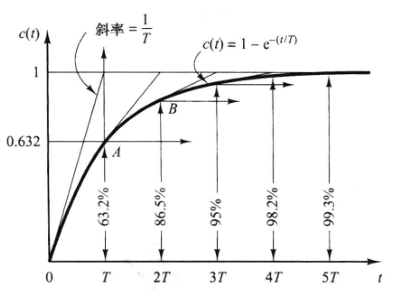
\includegraphics[width=8cm]{figures/6.png}
	\caption{一阶系统阶跃响应}
	\label{6}
\end{figure}

对应的时间常数$T$越小,系统的响应就越快。由图\ref{6}可以看出,当$t\ge4T$时,响应的误差将保持在2\%以内。$4T$可以作为响应时间的估值。

\subsubsection{单位斜坡响应}

单位斜坡函数的拉普拉斯变换为$1/s^2$,对应的输出可以表达为
\begin{gather*}
C(s)=\frac{1}{1+Ts}\frac{1}{s^2}=\frac{1}{s^2}-\frac{T}{s}+\frac{T^2}{1+Ts}\\
C(t)=\Laplace^{-1}[C(s)]=t-T+Te^{-t/T}
\end{gather*}

误差信号$e(t)$则为

\begin{gather*}
e(t)=r(t)-c(t)=T(1-e^{-t/T})\\
e(\infty)=T
\end{gather*}

\begin{figure}[!ht]
	\centering
	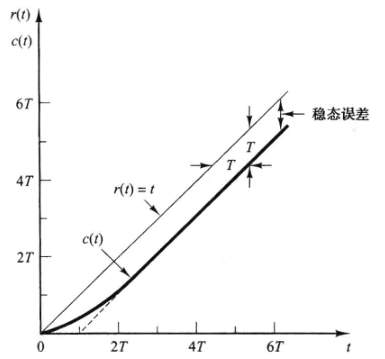
\includegraphics[width=8cm]{figures/7.png}
	\caption{一阶系统斜坡响应}
	\label{7}
\end{figure}

如图\ref{7},对于单位斜坡输入,其响应存在稳态误差$T$,因此时间常数越小,其稳态误差越小。

\subsubsection{单位脉冲响应}

单位脉冲输入信号可表示为狄拉克函数$\delta(t)$(其本质为泛函),其拉普拉斯变换为$R(s)=1$。系统的输出等于

\begin{gather*}
C(s)=\frac{1}{1+Ts}\\
c(t)=\Laplace^{-1}[C(s)]=\frac{1}{T}e^{-t/T}
\end{gather*}

\begin{figure}[!ht]
	\centering
	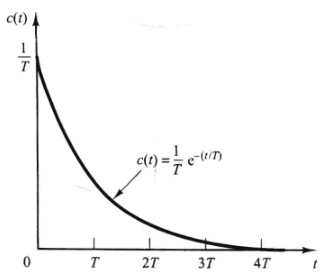
\includegraphics[width=8cm]{figures/8.png}
	\caption{一阶系统脉冲响应}
	\label{8}
\end{figure}

其响应曲线如图\ref{8}所示。

\subsubsection{线性定常系统特性}

对于线性定常系统,其输入信号求导,则输出信号也求导;其输入信号积分,其输出也积分。这是线性定常系统独有的特性,线性时变系统和非线性系统不具备这种特性。

\subsection{二阶系统}

\begin{figure}[!ht]
	\centering
	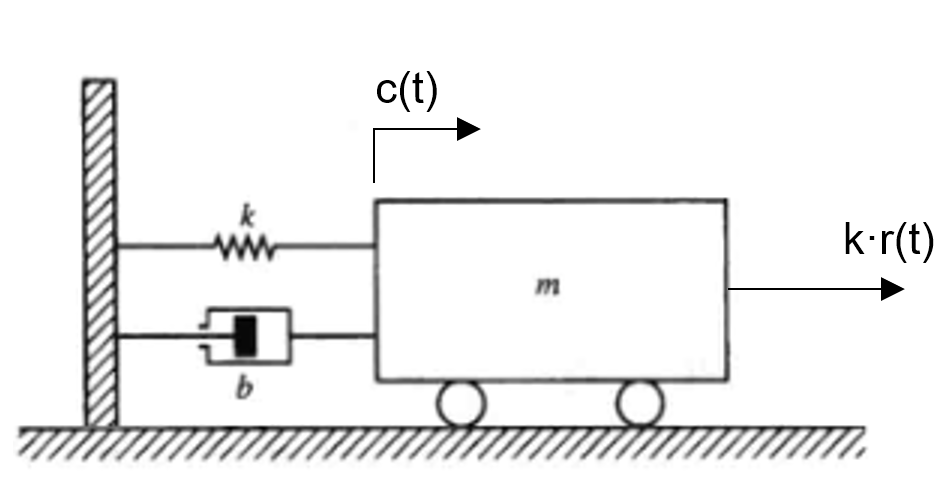
\includegraphics[width=8cm]{figures/9.png}
	\caption{二阶振动系统}
	\label{9}
\end{figure}

如图\ref{9}所示的振动系统,可以容易地列写出对应的微分方程与传递函数:

\begin{gather*}
m\ddot c+b\dot c+kc=kr(t)\\
(ms^2+bs+k)C(s)=kR(s)\\
\frac{C(s)}{R(s)}=\frac{k}{ms^2+bs+k}=\frac{k/m}{s^2+\frac{b}{m}s+\frac{k}{m}}
\end{gather*}

不难看出,传递函数具有两个极点,故此称为二阶系统。

可以将传递函数再改写为

\begin{equation*}
\frac{C(s)}{R(s)}=\frac{\frac{k}{m}}{\left[s+\frac{b}{2m}+\sqrt{(\frac{b}{m})^2-\frac{4k}{m}}\right]\left[s+\frac{b}{2m}-\sqrt{(\frac{b}{m})^2-\frac{4k}{m}}\right]}
\end{equation*}

当$b^2-2mk<0$时,闭环极点为共轭复数;当$b^2-2mk\ge0$时,闭环极点为实数。引入参量:

\begin{align*}
\omega_n^2&:=\frac{k}{m}\\
\sigma&:=\frac{b}{2m}=\zeta\omega_n
\end{align*}

式中,$\sigma$为衰减系数,$\omega_n$为无阻尼自然频率,$\zeta$为系统阻尼比。$\zeta$同时也是实际阻尼系数$b$与临界阻尼系数$b_c=2\sqrt{mk}$的比值。

传递函数可以改写成这样的形式:

\begin{equation*}
\frac{C(s)}{R(s)}=\frac{\omega_n^2}{s^2+2\zeta\omega_ns+\omega_n^2}
\end{equation*}

$\zeta=0$时,瞬态响应的振荡将永不停止;$0<\zeta<1$时,闭环极点为共轭复数,系统欠阻尼,响应会是振荡的;$\zeta=1$时,系统为临界阻尼系统;$\zeta>1$时,系统为过阻尼系统。

\subsubsection{单位阶跃响应}

对于单位阶跃信号的输入,其拉普拉斯变换为$R(s)=1/s$,对应的响应为

\begin{equation*}
C(s)=\frac{\omega_n^2}{(s^2+2\zeta\omega_ns+\omega_n^2)s}
\end{equation*}

\begin{enumerate}
	\item	欠阻尼情况($0<\zeta<1$)

	定义阻尼自然频率$\omega_d=\omega_n\sqrt{1-\zeta^2}$,则

	\begin{align*}
	C(s)&=\frac{\omega_n^2}{(s^2+2\zeta\omega_ns+\omega_n^2)s}\\
	&=\frac1s-\frac{s+2\zeta\omega_n}{(s^2+2\zeta\omega_ns+\omega_n^2)}\\
	&=\frac1s-\frac{s+\zeta\omega_n}{(s^2+2\zeta\omega_ns+\omega_n^2)}-\frac{\zeta\omega_n}{(s^2+2\zeta\omega_ns+\omega_n^2)}
	\end{align*}

	等式两边做拉普拉斯反变换,则有

	\begin{align*}
	c(t)&=\Laplace^{-1}[C(s)]\\
	&=1-e^{-\zeta\omega_nt}\cos\omega_dt-e^{-\zeta\omega_nt}\frac{\zeta}{\sqrt{1-\zeta^2}}\sin\omega_dt\\
	&=1-\frac{e^{-\zeta\omega_nt}}{\sqrt{1-\zeta^2}}\sin\left(\omega_dt+\arctan\frac{\sqrt{1-\zeta^2}}{\zeta}\right)
	\end{align*}

	可以看出,稳态时误差为$0$,瞬态振荡频率为阻尼自然频率$\omega_d$,它由无阻尼自然频率$\omega_n$和阻尼比$\zeta$决定。

	将$\zeta=0$代入,可以得到无阻尼振荡的响应

	\begin{equation*}
	c(t)=1-\cos\omega_nt
	\end{equation*}
	
	为无限期振荡。

	\item	临界阻尼情况($\zeta=1$)

	若两个极点相等,此时构成临界阻尼系统,

	\begin{gather*}
	C(s)=\frac{\omega_n^2}{(s+\omega_n)^2s}\\
	c(t)=1-e^{\omega_nt}(1+\omega_nt)
	\end{gather*}

	\item	过阻尼情况($\zeta>1$)

	此时极点为两个不等的负实数。

	\begin{align*}
	C(s)&=\frac{\omega_n^2}{\left(s+\zeta\omega_n+\omega_n\sqrt{\zeta^2-1}\right)\left(s+\zeta\omega_n-\omega_n\sqrt{\zeta^2-1}\right)}\\
	c(t)&=1+\frac{1}{2\sqrt{\zeta^2-1}\left(\zeta+\sqrt{\zeta^2-1}\right)}e^{-\left(\zeta+\sqrt{\zeta^2-1}\right)\omega_nt}\\
	&\hspace{2em}-\frac{1}{2\sqrt{\zeta^2-1}\left(\zeta-\sqrt{\zeta^2-1}\right)}e^{-\left(\zeta-\sqrt{\zeta^2-1}\right)\omega_nt}\\
	&=1+\frac{\omega_n}{2\sqrt{\zeta^2-1}}\left(\frac{e^{-s_1t}}{s_1}-\frac{e^{-s_2t}}{s_2}\right)
	\end{align*}

	式中,$s_1=\left(\zeta+\sqrt{\zeta^2-1}\right)\omega_n$,$s_2=\left(\zeta-\sqrt{\zeta^2-1}\right)\omega_n$。这是两个衰减的指数项。在$\zeta>>1$时,即阻尼极大,衰减项的影响将主要取决于衰减较慢的那一项;也就是说,当$\left|{s_2}\right|<<\left|{s_1}\right|$时,可以忽略$s_1$的影响。在这样的前提下,传递函数可近似表示为

	\begin{equation*}
	\frac{C(s)}{R(s)}=\frac{s_2}{s+s_2}
	\end{equation*}

	其单位阶跃响应为

	\begin{align*}
	C(s)&=\frac{s_2}{\left(s+s_2\right)s}\\
	c(t)&=1-e^{-\left(\zeta-\sqrt{\zeta^2-1}\right)\omega_nt}
	\end{align*}

\end{enumerate}

\begin{figure}[!ht]
	\centering
	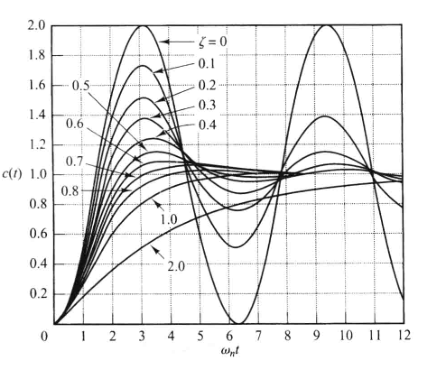
\includegraphics[width=8cm]{figures/10.png}
	\caption{不同阻尼比的单位阶跃响应曲线}
	\label{10}
\end{figure}

\subsubsection{瞬态响应指标}

对于单位阶跃输入信号的瞬态响应特性,用下列性能指标衡量,如图\ref{11}:

\begin{enumerate}
	\item	延迟时间$t_d$:响应曲线第一次达到稳态值一般所需的时间。
	\item	上升时间$t_r$:响应曲线从稳态值的10\%上升至90\%所需的时间,或是5\%上升至90\%,或是0\%上升至100\%所需的时间。
	\item	峰值时间$t_p$:响应曲线达到过调量的第一个峰值所需要的时间。
	\item	最大过调量$M_p$:从$1$开始计算的响应曲线的最大峰值为最大过调量。若响应稳态值不为$1$,则采用最大百分比过调量:
	\begin{equation*}
	\mbox{最大百分比过调量}=\frac{c(t_p)-c(\infty)}{c(\infty)}\times100\%
	\end{equation*}
	\item	调整时间$t_s$:响应曲线的稳态线上,稳态值的上下$2\%$或$5\%$以内作为允许误差范围;响应曲线达到并且永远处于这一误差范围内所需的时间即为调整时间。	
\end{enumerate}

\begin{figure}[!ht]
	\centering
	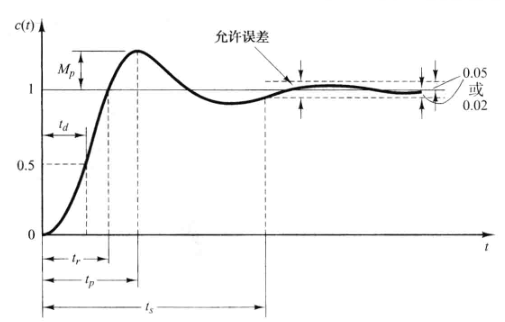
\includegraphics[width=8cm]{figures/11.png}
	\caption{单位阶跃响应的性能指标}
	\label{11}
\end{figure}

为了获得比较好的二阶系统瞬态响应特性,阻尼比必须选择在$0.4\sim0.8$之间。阻尼比过小会造成严重过调,而过大的阻尼比则会使系统响应变得缓慢。另一方面,最大过调量和上升时间存在Trade off关系,无法兼得。

\subsubsection{二阶系统的瞬态响应指标}

假设系统为欠阻尼二阶系统

\begin{enumerate}
	\item	上升时间$t_r$
	令$c(t_r)=1$,可得

	\begin{equation*}
	t_r=\frac{1}{\omega_d}\arctan\left(\frac{\omega_d}{-\sigma}\right)=\frac{\pi-\beta}{\omega_d}
	\end{equation*}

	其中$\beta$角的定义如图\ref{12}所示。

	\begin{figure}[!ht]
		\centering
		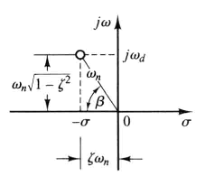
\includegraphics[width=8cm]{figures/12.png}
		\caption{$\beta$角的定义}
		\label{12}
	\end{figure}

	\item	峰值时间$t_p$
	令$dc(t)/dt=0$,可得

	\begin{align*}
	\sin\omega_dt_p=0\\
	t_p=\frac{\pi}{\omega_d}
	\end{align*}

	\item	最大过调量$M_p$

	最大过调量在峰值时间取到,直接代入$t_p$:

	\begin{align*}
	M_p&=c(t_p)-1\\
	&=e^{-(\sigma/\omega_d)\pi}\\
	&=e^{-(\zeta/\sqrt{1-\zeta^2})\pi}
	\end{align*}

	\item	调整时间$t_s$

	\begin{align*}
	t_s=4T=\frac{4}{\sigma}=\frac{4}{\zeta\omega_n}\hspace{2mm}\mbox{2\%误差标准}\\
	t_s=3T=\frac{3}{\sigma}=\frac{3}{\zeta\omega_n}\hspace{2mm}\mbox{5\%误差标准}
	\end{align*}
	
\end{enumerate}

经验公式:

对于二阶系统,要求$\delta=0.01y_\infty$时,有

\begin{equation*}
	\sigma\geq\frac{4.6}{t_s}
\end{equation*}

$\sigma$为极点距虚轴距离

定义$t_r$为$0.1y_\infty\rightarrow0.9y_\infty$,

\begin{equation*}
	\omega_n\geq\frac{1.8}{t_r}
\end{equation*}

$\omega_n$为极点距原点距离

给定最大过调量$M_p$,

\begin{equation*}
	\zeta\geq\frac{-\frac{\ln M_p}{\pi}}{\sqrt{1+\frac{\ln^2M_p}{\pi^2}}}
\end{equation*}

由图\ref{12}可知,$\cos\beta=\zeta,\quad\beta=\arccos\zeta$

\subsubsection{单位脉冲响应}

对于脉冲响应$r(t)=\delta(t)$,其拉普拉斯变换为$R(s)=1$,因此

\begin{align*}
C(s)&=\frac{\omega_n^2}{s^2+2\zeta\omega_ns+\omega_n^2}\\
c(t)&=\Laplace^{-1}[C(s)]
\end{align*}

\begin{enumerate}
	\item	$0\le\zeta<1$
	\begin{equation*}
	c(t)=\frac{\omega_n}{\sqrt{1-\zeta^2}}e^{-\zeta\omega_nt}\sin\omega_n\sqrt{1-\zeta^2}t
	\end{equation*}
	
	\item	$\zeta=1$
	\begin{equation*}
	c(t)=\omega_n^2te^{-\omega_nt}
	\end{equation*}

	\item	$\zeta>1$
	\begin{equation*}
	c(t)=\frac{\omega_n}{2\sqrt{\zeta^2-1}}e^{-(\zeta-\sqrt{\zeta^2-1})\omega_nt}-\frac{\omega_n}{2\sqrt{\zeta^2-1}}e^{-(\zeta+\sqrt{\zeta^2-1})\omega_nt}
	\end{equation*}
\end{enumerate}

对于临界阻尼和过阻尼的情况,单位脉冲响应总是非负的,$c(t)\ge0$。



\subsection{高阶系统}

对于高阶系统而言,往往考虑其主导极点(距离虚轴最近的一对共轭极点),二阶系统所给出的规律仍然具有指导意义。换言之,可以根据系统要求的瞬态响应指标,在复平面上给出``允许极点存在的位置''。事实上在处理高阶系统时,系统的频域响应更加重要。

\subsection{劳斯稳定判据}

劳斯稳定判据的作用是,对一个关于$s$的多项式方程,在无需实际求解这一方程,就可以判断系统的绝对稳定性。

多项式方程:

\begin{equation*}
a_0s^n+a_1s^{n-1}+\cdots+a_{n-1}s+a_n=0
\end{equation*}

其中$a_n\neq0$,即不存在零根。

\begin{itemize}
	\item	确保所有系数都是正的(如果全是负的则乘以$-1$到方程两边)。如果有负系数,则方程一定存在正根,即存在右半平面的极点,系统不稳定。
	\item	将多项式排列成下列形式:

	\begin{tabular}{llllll}
	$s^n$	&$a_0$	&$a_2$	&$a_4$	&$a_6$	& $\cdots$	\\
	$s^{n-1}$	&$a_1$	&$a_2$	&$a_3$	&$a_4$	& $\cdots$	\\
	$s^{n-2}$	&$b_1$	&$b_2$	&$b_3$	&$b_4$	& $\cdots$	\\
	$s^{n-3}$	&$c_1$	&$c_2$	&$c_3$	&$c_4$	& $\cdots$	\\
	$s^{n-4}$	&$d_1$	&$d_2$	&$d_3$	&$d_4$	& $\cdots$	\\
	$\vdots$	&$\vdots$	&$\vdots$\\
	$s^{2}$	&$e_1$	&$e_2$\\
	$s^{1}$	&$f_1$\\
	$s^{0}$	&$g_1$
	\end{tabular}

	其中,$b$,$c$,$d$,$e$等系数为

	\begin{equation*}
	\frac{\mbox{左下}\times\mbox{右上}-\mbox{左上}\times\mbox{右下}}{\mbox{左下}}
	\end{equation*}
	
	即

	\begin{align*}
	b_1&=\frac{a_1a_2-a_0a_3}{a_1}\\
	b_2&=\frac{a_1a_4-a_0a_5}{a_1}\\
	b_2&=\frac{a_1a_6-a_0a_7}{a_1}\\
	&\vdots\\
	c_1&=\frac{b_1a_3-a_1b_2}{b_1}\\
	c_2&=\frac{b_1a_5-a_1b_3}{b_1}\\
	c_3&=\frac{b_1a_7-a_1b_4}{b_1}\\
	&\vdots\\
	d_1&=\frac{c_1b_2-b_1c_2}{c_1}\\
	d_2&=\frac{c_1b_3-b_1c_3}{c_1}\\
	&\vdots
	\end{align*}
	
	直到用完所有行(没有数的地方视为$0$)。
\end{itemize}

劳斯稳定判据指出,多项式方程中,实部大于$0$的根数(右半平面极点),等于劳斯阵列中第一列系数符号的改变次数。所以,方程所有根在左半平面的充要条件是,劳斯阵列第一列所有项均为正数。

\begin{enumerate}
	\item	可以在列写劳斯阵列的过程中,把某一行整体乘以或除以一个正数,简化计算。
	\item	如果某一行的第一项等于零,但其余各项不等于零或没有其余项,则可以用一个很小的正数$\epsilon$代替该项。如果$\epsilon$上下的符号一致,则表明有一对纯虚根存在;若上下符号相反,则意味着一次变号。
	\item	如果某一行全为0,则意味着存在大小相等但互为相反数的一对根。这时,可以将最后一行非零行对应的系数构成一个辅助多项式,对该多项式求导,把求导后的系数作为新的行。
\end{enumerate}

\subsection{单位反馈控制系统中的稳态误差}

\subsubsection{控制系统分类}

开环传递函数

\begin{equation*}
G(s)=\frac{K(T_as+1)(T_bs+1)\cdots(T_ms+1)}{s^N(T_1s+1)(T_2s+1)\cdots(T_ps+1)}
\end{equation*}

$G(s)$分母中$s^N$项表示它在原点处有$N$重极点,称系统为$N$型系统(有别于$n$阶系统)。类型号数增加,系统精度会得到改善,但稳定性会随之下降。

\subsubsection{稳态误差}

由于开环传递函数为$G(s)$,且反馈为单位反馈,则闭环传递函数

\begin{equation*}
\frac{C(s)}{R(s)}=\frac{G(s)}{1+G(s)}
\end{equation*}

误差信号为

\begin{align*}
E(s)&=\frac{1}{1+G(s)}R(s)\\
e_{ss}&=\lim_{t\to\infty}e(t)=\lim_{s\to0}sE(s)=\lim_{s\to0}\frac{sR(s)}{1+G(s)}
\end{align*}

稳态误差小结:

\begin{small}
	\begin{tabular}{cccc}
		\centering
			&	阶跃输入$r(t)=1$	&	斜坡输入$r(t)=t$	&	加速度输入$r(t)=\frac12t^2$\\
		0型系统&	$\frac{1}{1+K}$	&$\infty$	&	$\infty$\\
		1型系统&$0$	&$\frac1K$&$\infty$\\
		2型系统&$0$	&$0$	&$\frac1K$
		\end{tabular}
\end{small}






\section{PID - 未完成(再包入第8章)}

所有PID控制器都是作用在误差信号$e(t)$上的。

\subsection{PID控制器}

\subsubsection{比例控制作用}

\begin{align*}
u(t)&=K_pe(t)\\
\frac{U(s)}{E(s)}&=K_p
\end{align*}

$K_p$称为比例增益。

\subsubsection{积分控制作用}

\begin{align*}
\frac{du(t)}{dt}&=K_ie(t)\\
u(t)&=K_i\int_0^te(t)dt\\
\frac{U(s)}{E(s)}&=\frac{K_i}{s}
\end{align*}

\subsubsection{比例+积分控制作用}

\begin{align*}
u(t)&=K_pe(t)+\frac{K_p}{T_i}\int_0^te(t)dt\\
\frac{U(s)}{E(s)}&=K_p\left(1+\frac{1}{T_is}\right)
\end{align*}

其中,$T_i$称为积分时间常数。

\subsubsection{比例+微分控制作用}

\begin{align*}
u(t)&=K_pe(t)+K_pT_d\frac{de(t)}{dt}\\
\frac{U(s)}{E(s)}&=K_p(1+T_ds)
\end{align*}

其中,$T_d$称为微分时间常数。

\subsubsection{比例+积分+微分控制作用}

\begin{align*}
u(t)&=K_pe(t)+\frac{K_p}{T_i}\int_0^te(t)dt+D_pT_d\frac{de(t)}{dt}\\
\frac{U(s)}{E(s)}&=K_p\left(1+\frac{1}{T_is}+T_ds\right)
\end{align*}

\subsection{积分和微分控制作用对系统性能的影响}

\subsubsection{积分控制作用}

如果传递函数中不存在积分器$1/s$,阶跃输入信号的响应一定会有稳态误差;通过引入积分控制系统,可以消除这种误差。

\subsubsection{比例控制}

对于阶跃输入信号,没有积分器时,一定存在稳态误差。

\begin{figure}[!ht]
	\centering
	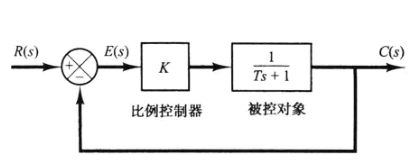
\includegraphics[width=8cm]{figures/13.png}
	\caption{比例控制系统}
	\label{13}
\end{figure}

如图\ref{13}所示的控制系统,

\begin{align*}
\frac{E(s)}{R(s)}&=\frac{R(s)-C(s)}{R(s)}=1-\frac{C(s)}{R(s)}=1-\frac{G(s)}{1+G(s)}=\frac{1}{1+G(s)}\\
E(s)&=\frac{1}{1+G(s)}R(s)=\frac{Ts+1}{Ts+1+K}\frac1s
\end{align*}

稳态误差为

\begin{equation*}
e_{ss}=\lim_{t\to\infty}e(t)=\lim_{s\to0}sE(s)=\lim_{s\to0}\frac{Ts+1}{Ts+1+K}=\frac{1}{K+1}
\end{equation*}

\subsubsection{积分控制}

积分控制可以消除稳态误差。如图\ref{14}所示的系统:

\begin{figure}[!ht]
	\centering
	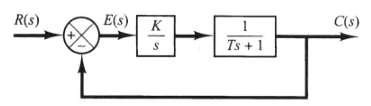
\includegraphics[width=8cm]{figures/14.png}
	\caption{积分控制系统}
	\label{14}
\end{figure}

\begin{align*}
\frac{C(s)}{R(s)}&=\frac{K}{s(Ts+1)+K}\\
{E(s)}&=\frac{s(Ts+1)}{s(Ts+1)+K}\frac1s
\end{align*}

稳态误差为

\begin{equation*}
e_{ss}=\lim_{t\to\infty}e(t)=\lim_{s\to0}sE(s)=\lim_{s\to0}\frac{s^2(Ts+1)}{Ts^2+s+K}\frac1s=0
\end{equation*}

\subsubsection{对转矩扰动的响应(比例控制)}

引入转矩扰动,如图\ref{15}所示,并令输入为$0$,即$R(s)=0$

\begin{figure}[!ht]
	\centering
	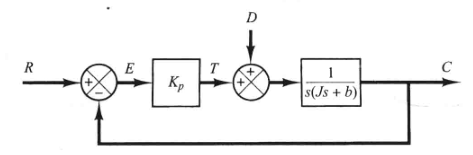
\includegraphics[width=8cm]{figures/15.png}
	\caption{转矩扰动(比例控制)}
	\label{15}
\end{figure}

考虑输出$C(s)$与扰动$D(s)$间的关系

\begin{equation*}
\frac{C(s)}{D(s)}=\frac{1}{Js^2+bs+K_p}
\end{equation*}

引起的误差

\begin{equation*}
\frac{E(s)}{D(s)}=\frac{R(s)-C(s)}{D(s)}=-\frac{1}{Js^2+bs+K_p}
\end{equation*}

假设扰动是一个幅值为$T_d$的阶跃扰动,$D(s)=T_d/s$,则稳态误差为

\begin{equation*}
e_{ss}=\lim_{t\to\infty}e(t)=\lim_{s\to0}sE(s)=\lim_{s\to0}\frac{-s}{Js^2+bs+K_p}\frac{T_d}{s}=-\frac{T_d}{K_p}
\end{equation*}

增大增益$K_p$可以减小稳态误差,但同时会导致系统响应的振荡加大。

\subsubsection{对转矩扰动的响应(比例+积分控制)}

在比例控制的基础上增加积分控制,可以消除稳态误差,如图\ref{16}所示:

\begin{figure}[!ht]
	\centering
	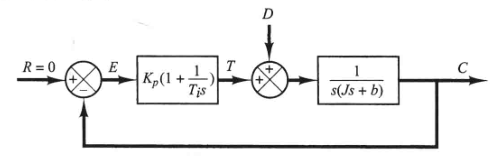
\includegraphics[width=8cm]{figures/16.png}
	\caption{转矩扰动(比例+积分控制)}
	\label{16}
\end{figure}

\begin{gather*}
\frac{C(s)}{D(s)}=\frac{s}{Js^3+bs^2+K_ps+\frac{K_p}{T_i}}\\
E(s)=-\frac{s}{Js^3+bs^2+K_ps+\frac{K_p}{T_i}}D(s)
\end{gather*}

如果特征方程

\begin{equation*}
Js^3+bs^2+K_ps+\frac{K_p}{T_i}=0
\end{equation*}

的根在左半平面,则系统稳定,稳态误差为

\begin{equation*}
e_{ss}=\lim_{t\to\infty}e(t)=\lim_{s\to0}sE(s)=\lim_{s\to0}\frac{-s^2}{Js^3+bs^2+K_ps+\frac{K_p}{T_i}}\frac{T_d}{s}=0
\end{equation*}

可以看出,稳态误差可以通过积分控制消除。在比例控制的基础上增加积分控制,会使二阶系统转变为三阶系统,如果$K_p$较大,特征方程的根需要注意保持在左半平面来保证系统稳定。

如果没有比例控制,仅靠积分控制,则系统总是不稳定的,因为特征方程$Js^3+bs^2+K=0$总有右半平面的根(韦达定理)。


\subsubsection{微分控制}

微分控制不能影响稳态误差,但是可以提前预知误差的变化,提前修正,增加系统阻尼,改善系统稳定性。

\subsubsection{惯性负载系统(比例控制)}

\begin{figure}[!ht]
	\centering
	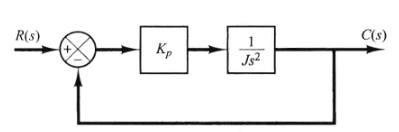
\includegraphics[width=8cm]{figures/17.png}
	\caption{惯性负载系统(比例控制)}
	\label{17}
\end{figure}

如图\ref{17}所示的惯性负载系统,其传递函数为:

\begin{equation*}
\frac{C(s)}{R(s)}=\frac{K_p}{Js^2+K_p}
\end{equation*}

特征方程:

\begin{equation*}
Js^2+K_p=0
\end{equation*}

显然方程有两个纯虚根,单位阶跃响应是无限期的持续振荡。

\subsubsection{惯性负载系统(比例+微分控制)}

\begin{figure}[!ht]
	\centering
	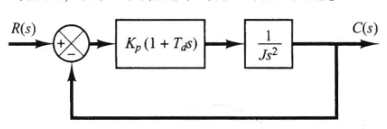
\includegraphics[width=8cm]{figures/18.png}
	\caption{惯性负载系统(比例+微分控制)}
	\label{18}
\end{figure}

如图\ref{18}所示,添加了微分控制,闭环传递函数为:

\begin{equation*}
\frac{C(s)}{R(s)}=\frac{K_p(1+T_ds)}{Js^2+K_pT_ds+K_p}
\end{equation*}

特征方程为:

\begin{equation*}
Js^2+K_pT_ds+K_p=0
\end{equation*}

特征方程的根都在左半平面,因此系统是稳定的。微分控制带来了阻尼效应。

\subsubsection{二级系统(比例+微分控制)}

\begin{figure}[!ht]
	\centering
	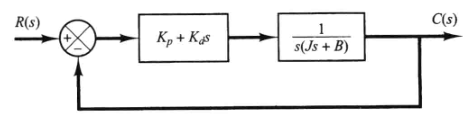
\includegraphics[width=8cm]{figures/19.png}
	\caption{二阶系统(比例+微分控制)}
	\label{19}
\end{figure}

如图\ref{19}所示的二阶系统,其闭环传递函数:

\begin{equation*}
\frac{C(s)}{R(s)}=\frac{K_p+K_ds}{Js^2+(B+K_d)s+K_p}
\end{equation*}

前文已经推导过,对于单位斜坡输入,其稳态误差为

\begin{equation*}
e_{ss}=\frac{B}{K_p}
\end{equation*}

阻尼比为

\begin{equation*}
\zeta=\frac{B+K_p}{2\sqrt{K_pJ}}
\end{equation*}

为了减小稳态误差,可以提高增益$K_p$、减小$B$,同时为了补偿阻尼比,减小振荡,还应同步地增大$K_d$,最终使阻尼比$\zeta$落在$0.4\sim0.7$的可以接受的范围内。





\section{根轨迹法}

\begin{figure}[!ht]
    \centering
    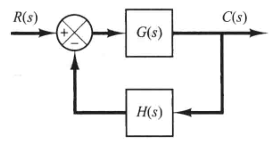
\includegraphics[width=8cm]{figures/20.png}
    \caption{闭环系统}
    \label{20}
\end{figure}

考虑如图\ref{20}所示的闭环控制系统,其传递函数为

\begin{equation*}
    \frac{C(s)}{R(s)}=\frac{G(s)}{1+G(s) H(s)}
\end{equation*}

令等式右端分母为$0$,得到特征方程:

\begin{equation*}
    1+G(s) H(s)=0
\end{equation*}

由于在$G(s)$或$H(s)$中往往存在增益$K$,可以进一步把特征方程改写为

\begin{equation*}
    1+\frac{K\left(s+z_{1}\right)\left(s+z_{2}\right) \cdots\left(s+z_{m}\right)}{\left(s+p_{1}\right)\left(s+p_{2}\right) \cdots\left(s+p_{n}\right)}=0
\end{equation*}

所谓根轨迹图,即为增益参数$K$由0变到无穷大时,闭环极点的轨迹。

典型步骤:

\begin{enumerate}
    \item 确定实轴上的根轨迹
    
    首先画出所有的开环极点与开环零点,随后根据辐角条件,确定实轴上的根轨迹。

    \item 确定渐近线
    
    \begin{align*}
        \sigma&=\frac{\sum\mbox{poles}-\sum\mbox{zeros}}{n-m}\\
        \eta_k&=\frac{(2k+1)\pi}{n-m}\quad k=0,1,2,\cdots ,n-m
    \end{align*}

    得到的$\sigma$即为渐近线与实轴的交点,$\eta_k$则是渐近线可以取到的角度。

    \item 确定分离点与会合点
    
    首先将特征方程$1+G(s) H(s)=0$化为$K=K(s)$的形式,即

    \begin{equation*}
        K=-\frac{\left(s+p_{1}\right)\left(s+p_{2}\right) \cdots\left(s+p_{n}\right)}{\left(s+z_{1}\right)\left(s+z_{2}\right) \cdots\left(s+z_{m}\right)}
    \end{equation*}

    随后令$dK/ds=0$,对应得到的$s$取值即为实轴上分离点或会合点的位置。把这个$s$代回$K=K(s)$,就可以得到该点对应的增益参数$K$。另一个方法是将式子化为关于$s$的多项式方程$f(s)=0$,由于在分离点或会合点,相当于这个方程在此处取到重根,则可以联立$df/ds=0$与$f(s)=0$,解出对应的$K$和$s$。

    \item 确定根轨迹与虚轴的交点
    
    由于极点位于虚轴上时,系统处于临界稳定状态,可以通过劳斯稳定判据确定此时对应的$K$值。使劳斯阵列第一列上的项等于零,就能得到该状态对应的$K$,再通过辅助方程,求解根轨迹与虚轴的交点。

    \item 确定极点出射角与零点入射角
    
    将试验点取在非常靠近零点/极点的地方,利用辐角条件,即可得到对应的出射/入射角度。根轨迹从极点出发,结束于零点或无穷远点处。

\end{enumerate}

MatLab中,可以直接利用\textit{rlocus}函数来绘制根轨迹图。

\begin{lstlisting}
    rlocus(num,den)
\end{lstlisting}

如图\ref{21},是一个绘制根轨迹图的例子,特征方程为:

\begin{equation*}
    0.1s^3+1.15s^2+2.5s+K(0.1s+1)=0
\end{equation*}

\begin{figure}[!ht]
    \centering
    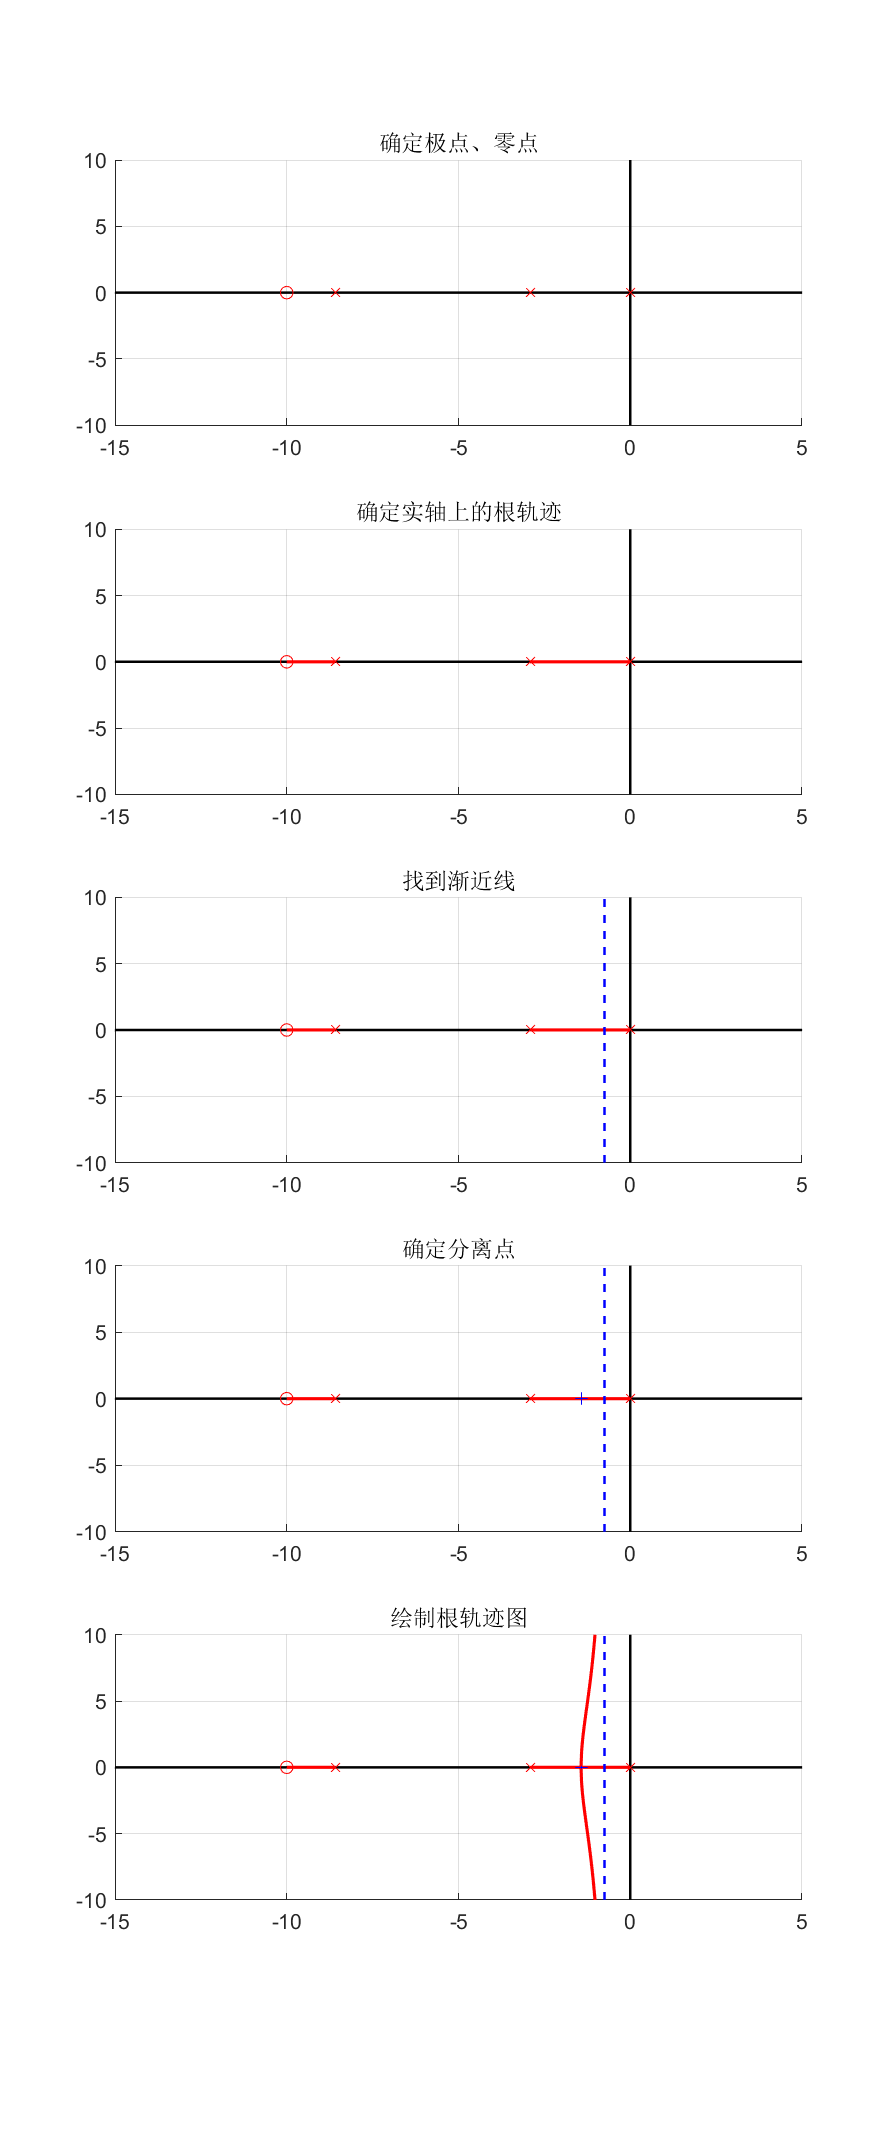
\includegraphics[width=0.5\linewidth]{figures/21.png}
    \caption{绘制根轨迹图}
    \label{21}
\end{figure}
\section{频响分析法}

系统对正弦输入信号的稳态响应称为频率响应。通过改变输入信号的频率,考察系统产生的响应,可以作为分析和设计控制系统的重要依据。

正弦传递函数就是把系统传递函数中的$s$用$j\omega$代替所得到的函数,其中$\omega$为频率,单位为$rad/s$。当用$circ/s$为单位测量频率时,频率用$f$来表示,$\omega=2\pi f$。

传递函数可以表示为相位与辐角的形式

\begin{equation*}
    G(j\omega)=Me^{j\phi}=M\phase{\phi}
\end{equation*}

稳定的线性定常系统在收到正弦信号的输入后,在稳态时将会输出一个和输入信号频率相同的正弦输出信号。然而输出的幅值和相位一般和输入信号存在差异,这由正弦传递函数决定。

\begin{align*}
    |G(j \omega)|&=\left|\frac{Y(j \omega)}{X(j \omega)}\right|\\ 
    \phase{G(j \omega)}&=\phase{\frac{Y(j \omega)}{X(j \omega)}}
\end{align*}

\subsection{伯德图}

伯德图有两幅图组成,一幅是正弦传递函数幅值的对数坐标图,另一幅是相角图。两幅图的横坐标都是频率的对数。

对数幅值的表达式为$20\log\left|G(j\omega)\right|$,所得到的单位是分贝$dB$。

用MATLAB绘制伯德图的命令是

\begin{lstlisting}
    bode(num,den)
    bode(sys)
    [mag,phase,w]=bode(num,den,w)
\end{lstlisting}

得到的伯德图如图\ref{22}所示。

\begin{figure}[!ht]
    \centering
    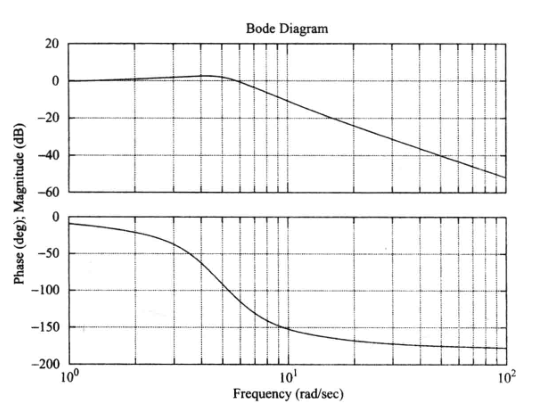
\includegraphics[width=8cm]{figures/22.png}
    \caption{伯德图}
    \label{22}
\end{figure}

\subsection{奈奎斯特图}

奈奎斯特图也称为极坐标图,是当$\omega$由零变到无穷大时,表示在极坐标上$G(j\omega)$的幅值和相角的关系图。如图\ref{23}所示。

\begin{figure}[!ht]
    \centering
    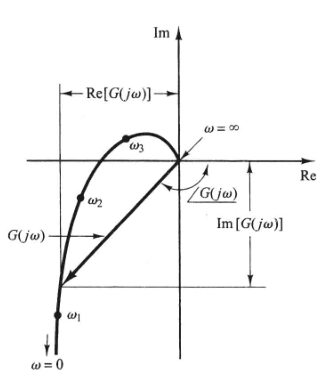
\includegraphics[width=8cm]{figures/23.png}
    \caption{奈奎斯特图}
    \label{23}
\end{figure}

用MATLAB绘制奈奎斯特图的命令是

\begin{lstlisting}
    nyquist(num,den)
    nyquist(sys)
    [re,im,w]=nyquist(num,den,w)
\end{lstlisting}

\subsection{奈奎斯特稳定判据}

\textbf{柯西辐角原理}

对于传递函数

\begin{equation*}
    \frac{C(s)}{R(s)}=\frac{G(s)}{1+G(s)H(s)}
\end{equation*}

系统稳定的条件为特征方程

\begin{equation*}
    1+G(s)H(s)=0
\end{equation*}

的根均位于$s$左半平面。

通过分析映射后的辐角,如图\ref{24}所示,不难得到结论:在$s$平面内封闭曲线顺时针包围$F(s)$的零点一次,则映射后的封闭曲线在$F(s)$平面内顺时针包围原点一次。

\begin{figure}[!ht]
    \centering
    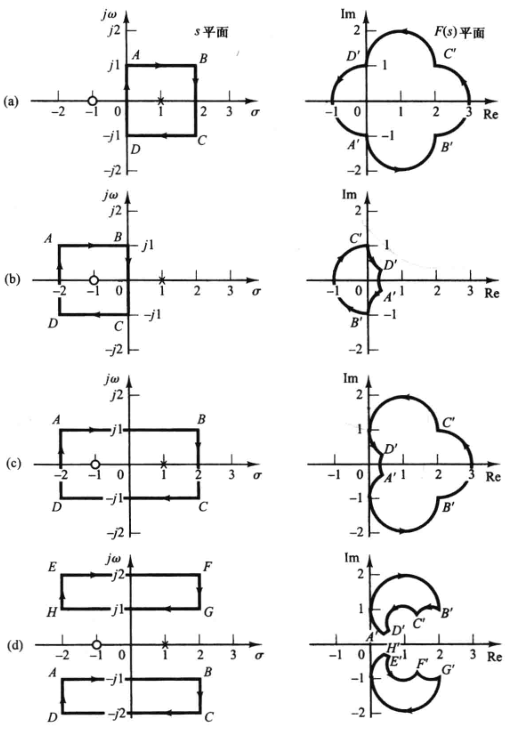
\includegraphics[width=8cm]{figures/24.png}
    \caption{$s$平面封闭曲线映射到$F(s)$平面的结果}
    \label{24}
\end{figure}

更一般地,则可以推广到柯西辐角原理:

\begin{equation*}
    N=Z-P
\end{equation*}

其中,$P$为$s$平面封闭曲线包围的$F(s)$极点数,$Z$为$s$平面封闭曲线包围的$F(s)$零点数,$N$为映射后$F(s)$平面封闭曲线顺时针包围原点的次数(若为负则代表逆时针包围)。

那么回到闭环传递函数与特征多项式

\begin{align*}
    T_0(s)&=\frac{C(s)G(s)}{1+C(s)G(s)}\\ 
    F(s)&=1+C(s)G(s)
\end{align*}

易得$F(s)$的零点,就对应着$T_0(s)$的极点。不妨假设$\Lambda_0(s)=C(s)G(s)$中分母的次数大于分子的次数,因此

\begin{equation*}
    \lim_{|s|\rightarrow\infty}F(s)=1
\end{equation*}

\begin{figure}[!ht]
    \centering
    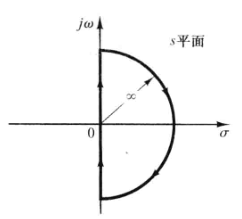
\includegraphics[width=8cm]{figures/25.png}
    \caption{$s$平面内封闭曲线的选取}
    \label{25}
\end{figure}

选取如图\ref{25}的封闭曲线,假设在虚轴上不存在零极点,则该曲线包围了右边平面$F(s)$全部的零极点。因此,如果我们知道了$\Lambda_0(s)$右半平面的极点数$P$,即可以通过观察$\Lambda_0(s)$奈奎斯特图中围绕点$(-1,j0)$点的次数$N$,就能得到$F(s)$的零点数$Z$。

因此,奈奎斯特稳定判据可以简单地表述为:如果开环传递函数$G(s)H(s)$在右半平面内有$P$个极点,则当$\omega$从$-\infty$变到$\infty$时,$G(j\omega)H(j\omega)$逆时针包围$(-1,j0)$点$P$次时,闭环系统稳定。

\subsection{$G(s)H(s)$含有位于虚轴上零极点的特殊情况}

当在虚轴上有开环传递函数的零极点时,就需要对$s$平面上的封闭曲线进行一定的改造,如图\ref{26}所示。

\begin{figure}[!ht]
    \centering
    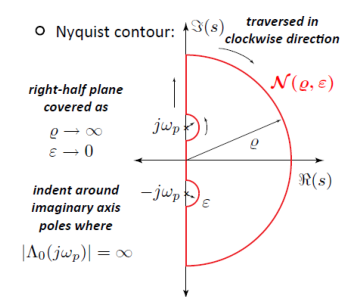
\includegraphics[width=8cm]{figures/26.png}
    \caption{$s$平面封闭曲线的改造}
    \label{26}
\end{figure}

例如:考虑开环传递函数

\begin{equation*}
    G(s)H(s)=\frac{K}{s(Ts+1)}
\end{equation*}

在$G(s)H(s)$平面上,对应$s=j0+$和$s=j0-$的点分别为$-j\infty$和$+j\infty$。在半径$\epsilon$的半圆轨迹上,如图\ref{27}所示,可以表示为

\begin{equation*}
    s=\epsilon e^{i\theta}\quad \theta=-90^\circ\rightarrow+90^\circ
\end{equation*}

\begin{figure}[!ht]
    \centering
    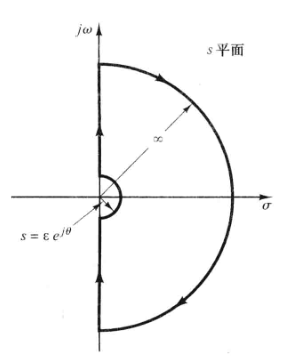
\includegraphics[width=8cm]{figures/27.png}
    \caption{改造后曲线}
    \label{27}
\end{figure}

对应的$G(s)H(s)$变为

\begin{equation*}
    G\left(\varepsilon \mathrm{e}^{j \theta}\right) H\left(\varepsilon \mathrm{e}^{j \theta}\right)=\frac{K}{\varepsilon \mathrm{e}^{j \theta}}=\frac{K}{\varepsilon} \mathrm{e}^{-j \theta}
\end{equation*}

可以得到对应的$G(s)H(s)$平面的封闭曲线如图\ref{28}所示。由于$s$右半平面没有极点,$G(s)H(s)$轨迹也不包围$(-1,j0)$点,因此$1+G(s)H(s)$没有位于右半平面的零点,系统稳定。

\begin{figure}[!ht]
    \centering
    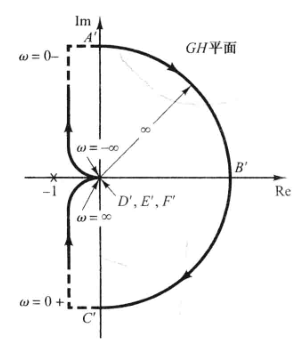
\includegraphics[width=8cm]{figures/28.png}
    \caption{$G(s)H(s)$平面上的封闭曲线}
    \label{28}
\end{figure}

\subsection{相对稳定性分析}

为了表示稳定系统的稳定程度,可以定义一系列相对稳定性参数。

\textbf{相位裕量}

开环传递函数的幅值$|G(j\omega)|$等于1时,此处的相角$\Phi$加$180^\circ$即为相位裕量

\begin{equation*}
    \gamma=180^\circ + \Phi\quad\mbox{Phase Margin, }M_f
\end{equation*}

\textbf{增益裕量}

在相角等于$-180^\circ$的频率上,幅值$|G(j\omega)|$的倒数称为增益裕量

\begin{equation*}
    K_g=\frac{1}{|G(j\omega)|}
\end{equation*}

一般以分贝表示

\begin{equation*}
    K_g(dB)=20\log K_g=-20\log |G(j\omega)|\quad\mbox{Gain Margin, }M_g
\end{equation*}

\textbf{灵敏度峰值}

以$-1,j0$为圆心,与Nyquist轨迹不相交的最大的圆的半径的倒数。

\begin{equation*}
    \frac{1}{\eta}=\frac{1}{\min|1+\Lambda_0(j\omega)|}\quad\mbox{Sensitivity Peak}
\end{equation*}

图\ref{29}展示了相对稳定性参数在伯德图和奈奎斯特图中的意义。

\begin{figure}[!ht]
    \centering
    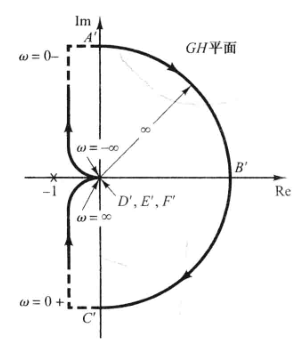
\includegraphics[width=8cm]{figures/29.png}
    \caption{相位裕量和增益裕量}
    \label{29}
\end{figure}
\section{拉普拉斯变换表与部分分式展开}

拉普拉斯变换:

\begin{equation*}
    \mathscr{L}[f(t)]=F(s)=\int_{0}^{\infty} \mathrm{e}^{-s t} \mathrm{d} t[f(t)]=\int_{0}^{\infty} f(t) \mathrm{e}^{-s t} \mathrm{d} t
\end{equation*}

拉普拉斯逆变换:

\begin{equation*}
    \mathscr{L}^{-1}[F(s)]=f(t)=\frac{1}{2 \pi j} \int_{c-j \infty}^{c+j \infty} F(s) \mathrm{e}^{s t} \mathrm{d} s, \quad t>0
\end{equation*}

拉普拉斯变换表


\begin{centering}
    \renewcommand{\arraystretch}{2}
    \begin{longtable}{|c|c|}
        \hline
            \boldmath{$f(t)$}\unboldmath &   \boldmath$F(s)$\unboldmath\\ \hline
            $\delta(t)$ &   $1$ \\  \hline
            $1(t)$  &   $\frac{1}{s}$\\  \hline
            $t$ &   $\frac{1}{s^2}$\\  \hline
            $\frac{t^{n-1}}{(n-1) !} \quad(n=1,2,3, \cdots)$    &   $\frac{1}{s^{n}}$\\  \hline
            $t^{n} \quad(n=1,2,3, \cdots)$  &   $\frac{n !}{s^{n+1}}$   \\  \hline
            $e^{-a t}$  &   $\frac{1}{s+a}$ \\  \hline
            $t e^{-a t}$    &   $\frac{1}{(s+a)^{2}}$   \\  \hline
            $\frac{1}{(n-1) !} t^{n-1} \mathrm{e}^{-a t} \quad(n=1,2,3, \cdots)$    &   $\frac{1}{(s+a)^{n}}$   \\  \hline
            $t^{n} \mathrm{e}^{-a t} \quad(n=1,2,3, \cdots)$    &   $\frac{n !}{(s+a)^{n+1}}$   \\  \hline
            $\sin \omega t$ &   $\frac{\omega}{s^{2}+\omega^{2}}$   \\  \hline
            $\cos \omega t$ &   $\frac{s}{s^{2}+\omega^{2}}$    \\  \hline
            $\sinh \omega t$    &   $\frac{\omega}{s^{2}-\omega^{2}}$   \\  \hline
            $\cosh \omega t$    &   $\frac{s}{s^{2}-\omega^{2}}$    \\  \hline
            $\frac{1}{a}\left(1-\mathrm{e}^{-a t}\right)$   &   $\frac{1}{s(s+a)}$  \\  \hline
            $\frac{1}{b-a}\left(\mathrm{e}^{-a t}-\mathrm{e}^{-b t}\right)$ &   $\frac{1}{(s+a)(s+b)}$  \\  \hline
            $\frac{1}{b-a}\left(b \mathrm{e}^{-b t}-a \mathrm{e}^{-a t}\right)$ &  $\frac{s}{(s+a)(s+b)}$   \\  \hline
            $\frac{1}{a b}\left[1+\frac{1}{a-b}\left(b \mathrm{e}^{-a t}-a \mathrm{e}^{-b t}\right)\right]$ &   $\frac{1}{s(s+a)(s+b)}$ \\  \hline
            $\frac{1}{a^{2}}\left(1-\mathrm{e}^{-a t}-a t \mathrm{e}^{-a t}\right)$ &   $\frac{1}{s(s+a)^{2}}$  \\  \hline
            $\frac{1}{a^{2}}\left(at-1+\mathrm{e}^{-at}\right)$& $\frac{1}{s^{2}(s+a)}$\\   \hline
            $\mathrm{e}^{-a t} \sin \omega t$   &   $\frac{\omega}{(s+a)^{2}+\omega^{2}}$   \\  \hline
            $\mathrm{e}^{-a t} \cos \omega t$   &   $\frac{s+a}{(s+a)^{2}+w^{2}}$   \\  \hline
            $\frac{\omega_{n}}{\sqrt{1-\zeta^{2}}} \mathrm{e}^{-\zeta \omega_{n} t} \sin \omega_{n} \sqrt{1-\zeta^{2}} t \quad(0<\zeta<1)$  &   $\frac{\omega_{n}^{2}}{s^{2}+2 \zeta \omega_{n} s+\omega_{n}^{2}}$  \\  \hline
            \begin{tabular}{c}$-\frac{1}{\sqrt{1-\zeta^{2}}} \mathrm{e}^{-\zeta \omega_{n} t} \sin \left(\omega_{n} \sqrt{1-\zeta^{2}} t-\phi\right)$\\ $\phi=\arctan \frac{\sqrt{1-\zeta^{2}}}{\zeta}$\\ $(0<\zeta<1,0<\phi<\pi / 2)$\end{tabular}   &   $\frac{s}{s^{2}+2 \zeta \omega_{n} s+\omega_{n}^{2}}$    \\  \hline
            \begin{tabular}{c}$1-\frac{1}{\sqrt{1-\zeta^{2}}} \mathrm{e}^{-\zeta \omega_{n} t} \sin \left(\omega_{n} \sqrt{1-\zeta^{2}} t+\phi\right)$\\ $\phi=\arctan \frac{\sqrt{1-\zeta^{2}}}{\zeta}$\\ $(0<\zeta<1,0<\phi<\pi / 2)$\end{tabular}   &   $\frac{s}{s(s^{2}+2 \zeta \omega_{n} s+\omega_{n}^{2})}$ \\
            $1-\cos\omega t$    & $\frac{\omega^2}{s(s^2+\omega^2)}$    \\   \hline
            $\omega t-\sin\omega t$    & $\frac{\omega^3}{s^2(s^2+\omega^2)}$       \\  \hline
            $\sin\omega t-\omega t \cos\omega t$    &   $\frac{2\omega^3}{(s^2+\omega^2)^2}$    \\  \hline
            $\frac{1}{2\omega}t\sin\omega   t$ & $\frac{s}{(s^2+\omega^2)^2}$   \\  \hline
            $t\cos\omega t$ & $\frac{s^2-\omega^2}{(s^2+\omega^2)^2}$   \\  \hline
            $\frac{1}{\omega_2^2-\omega_1^2}(\cos\omega_1t-\cos\omega_2t)\quad(\omega_1^2\neq\omega_2^2)$  & $\frac{s}{(s^2+\omega_1^2)(s^2+\omega_2^2)}$  \\   \hline
            $\frac{1}{2\omega}(\sin\omega t+\omega t \cos \omega t)$  & $\frac{s^2}{(s^2+\omega^2)^2}$  \\
        \hline
    \end{longtable}
\end{centering}

\newpage
拉普拉斯变换性质表

\begin{centering}
    \renewcommand{\arraystretch}{2}
    \begin{longtable}{|c|}
        \hline
        $\mathscr{L}[A f(t)]=A F(s)$\\  \hline
        $\mathscr{L}\left[f_{1}(t) \pm f_{2}(t)\right]=F_{1}(s) \pm F_{2}(s)$\\  \hline
        $\mathscr{L}_{ \pm}\left[\frac{\mathrm{d}}{\mathrm{d} t} f(t)\right]=s F(s)-f(0 \pm)$\\  \hline
        $\mathscr{L}_{ \pm}\left[\frac{\mathrm{d}^{2}}{\mathrm{d} t^{2}} f(t)\right]=s^{2} F(s)-s f(0 \pm)-\dot{f}(0 \pm)$\\  \hline
        $\mathscr{L}_{ \pm}\left[\frac{\mathrm{d}^{n}}{\mathrm{d} t^{n}} f(t)\right]=s^{n} F(s)-\sum_{k=1}^{n} s^{n-k} f(0 \pm)$\\  \hline
        $\mathscr{L}_{ \pm}\left[\int f(t) \mathrm{d} t\right]=\frac{F(s)}{s}+\frac{1}{s}\left[\int f(t) \mathrm{d} t\right]_{t=0 \pm}$\\  \hline
        $\Laplace_{\pm}\left[\int\cdots\int f(t)(\mathrm{d}t)^n\right]=\frac{F(s)}{s^n}+\sum_{k=1}^n\frac{1}{s^{n-k+1}}\left[\int\cdots\int f(t)(\mathrm{d}t)^k\right]_{t=0\pm}$\\  \hline
        $\mathscr{L}\left[\int_{0}^{t} f(t) \mathrm{d} t\right]=\frac{F(s)}{s}$\\  \hline
        $\int_{0}^{\infty} f(t) \mathrm{d} t=\lim _{s \rightarrow 0} F(s)$ (前提$\int_{0}^{\infty} f(t) \mathrm{d} t$存在)\\  \hline
        $\mathscr{L}\left[\mathbf{e}^{-\alpha t} f(t)\right]=F(s+a)$\\  \hline
        $\mathscr{L}[f(t-\alpha) 1(t-\alpha)]=\mathrm{e}^{-\alpha s} F(s) \quad \alpha \geq 0$\\  \hline
        $\mathscr{L}[t f(t)]=-\frac{\mathrm{d} F(s)}{\mathrm{d} s}$\\  \hline
        $\mathscr{L}\left[t^{2} f(t)\right]=\frac{\mathrm{d}^{2}}{\mathrm{d} s^{2}} F(s)$\\  \hline
        $\mathscr{L}\left[t^{n} f(t)\right]=(-1)^{n} \frac{\mathrm{d}^{n}}{\mathrm{d} s^{n}} F(s) \quad(n=1,2,3, \cdots)$\\  \hline
        $\mathscr{L}\left[\frac{1}{t} f(t)\right]=\int_{s}^{\infty} F(s) d s$ (前提$\lim _{t \rightarrow 0} \frac{1}{t} f(t)$存在)\\  \hline
        $\mathscr{L}\left[f\left(\frac{1}{a}\right)\right]=a F(a s)$\\  \hline
        $\mathscr{L}\left[\int_{0}^{t} f_{1}(t-\tau) f_{2}(\tau) \mathrm{d} \tau\right]=F_{1}(s) F_{2}(s)$\\  \hline
        $\mathscr{L}[f(t) g(t)]=\frac{1}{2 \pi j} \int_{c-j \infty}^{c+j \infty} F(p) G(s-p) \mathrm{d} p$\\  \hline
        $f(0+)=\lim _{t \rightarrow 0+} f(t)=\lim _{s \rightarrow \infty} s F(s)$\\  \hline
        $f(\infty)=\lim _{t \rightarrow \infty} f(t)=\lim _{s \rightarrow 0} s F(s)$ (前提系统稳定)\\
        \hline
    \end{longtable}
\end{centering}

\newpage

部分分式展开

$a_k$为$s=-p_k$处的留数:

\begin{gather*}
    F(s)=\frac{B(s)}{A(s)}=\frac{a_{1}}{s+p_{1}}+\frac{a_{2}}{s+p_{2}}+\cdots+\frac{a_{n}}{s+p_{n}}\\
    a_{k}=\left[\left(s+p_{k}\right) \frac{B(s)}{A(s)}\right]_{s=-p_{k}}
\end{gather*}

多重极点情况(例)

\begin{gather*}
    F(s)=\frac{s^{2}+2 s+3}{(s+1)^{3}}\\
    F(s)=\frac{B(s)}{A(s)}=\frac{b_{1}}{s+1}+\frac{b_{2}}{(s+1)^{2}}+\frac{b_{3}}{(s+1)^{3}}\\
    \begin{aligned} b_{3} &=\left[(s+1)^{3} \frac{B(s)}{A(s)}\right]_{s=-1} \\ &=\left(s^{2}+2 s+3\right)_{s=-1} \\ &=2 \end{aligned}\\
    \begin{aligned} b_{2} &=\left\{\frac{\mathrm{d}}{\mathrm{d} s}\left[(s+1)^{3} \frac{B(s)}{A(s)}\right]\right\}_{s=-1} \\ &=\left[\frac{\mathrm{d}}{\mathrm{d} s}\left(s^{2}+2 s+3\right)\right]_{s=-1} \\ &=(2 s+2)_{s=-1} \\ &=0 \end{aligned}\\
    \begin{aligned} b_{1} &=\frac{1}{2 !}\left\{\frac{\mathrm{d}^{2}}{s^{2}}\left[(s+1)^{3} \frac{B(s)}{A(s)}\right]\right\}_{s=-1} \\ &=\frac{1}{2 !}\left[\frac{\mathrm{d}^{2}}{s^{2}}\left(s^{2}+2 s+3\right)\right]_{s=-1} \\ &=\frac{1}{2}(2)=1 \end{aligned}\\
    \begin{aligned} f(t) &=\mathscr{L}^{-1}[F(s)] \\ &=\mathscr{L}^{-1}\left[\frac{1}{s+1}\right]+\mathscr{L}^{-1}\left[\frac{0}{(s+1)^{2}}\right]+\mathscr{L}^{-1}\left[\frac{2}{(s+1)^{3}}\right] \\ &=\mathrm{e}^{-t}+0+t^{2} \mathrm{e}^{-t} \\ &=\left(1+t^{2}\right) \mathrm{e}^{-t}, \quad t \geq 0 \end{aligned}
\end{gather*}




\end{document}